\documentclass[11pt]{article}
%Gummi|065|=)

\usepackage[margin=2cm]{geometry}

\usepackage[T1]{fontenc}
\usepackage{helvet}
\renewcommand{\familydefault}{\sfdefault}
% Font

\renewcommand{\baselinestretch}{1.5}
% Line spacing

\usepackage{lineno}
\usepackage{setspace}
\usepackage{blindtext}
\usepackage{graphicx}
\usepackage{caption}

\begin{document}

\begin{titlepage}
	\begin{center} % Align to the centre
		\vspace*{1cm} % Leave a gap between the top of the page and the text.
		
		\large
		Imperial College London
		
		\vspace{0.5cm}
		\large
		CMEE MRes Project Proposal
		
		\vspace{1.5cm}
		\LARGE
		\textbf{Integrating Body Size or Temperature Scaling with the Neutral Theory of Biodiversity}\\ % Bold font
		\emph{(a draft title)}
		
		\vspace{1.5cm}
		
		\large
		\textbf{Calum Pennington}
		
		\vspace{1.5cm}
		\textbf{Supervisors}\\
		Dr. James Rosindell (j.rosindell@imperial.ac.uk)\\
		Dr. Samraat Pawar (s.pawar@imperial.ac.uk)
		
		\vspace{1.5cm}
		\textbf{Committee Members (TBC)}\\
		Prof. Tim Barraclough\\
		Dr. Rob Ewers
		
		\vfill
		
		9 December 2016
		
	\end{center}
		
\end{titlepage}

\linenumbers

\section*{Proposal's Remit}
This is an initial proposal, put together at an early stage in the learning process. It will develop further, as my knowledge and understanding of this exciting and intriguing area grows.

\section*{Background}
\subsection*{Neutral Biodiversity Theory}
Neutral Theory assumes that all individuals in a community are ecologically identical \cite{rosindell2011unified}. Its success at reproducing biodiversity patterns suggests that demographic stochasticity, rather than the differences among species, is the key influence on diversity \cite{o2009integrative}. Neutral Theory is a drastic simplification of reality. It provides a null model, from which to test whether the added complexity of other mechanisms can explain biodiversity.\\
\\
\emph{Key parameters of a neutral model: random death, speciation, and dispersal.}

\subsection*{Allometry and Metabolic Scaling}
Body size determines an organism's metabolic rate - the rate at which it expends energy (e.g. for growth and reproduction). Thus, body size has a big impact on the structure and function of communities and ecosystems. Specifically, metabolic rate scales as a power function with body mass \cite{sibly2012metabolic}.\\

Scaling relationships are a powerful set of generalisations, which essentially assume all species of the same size behave the same way. Like Neutral Theory, they give a quantitative starting point for understanding the structure of a complex system. Fascinated by the simplicity and success of these approaches, I am drawn to investigating the links between them, and the next layer of complexity.

\subsection*{Overarching Purpose}
\emph{Fundamental aim:} make simple assumptions about complex systems to see what can be explained by models.\\
\\
\emph{Context:} quantify the effects of body size/temperature on biodiversity patterns, relative to demographic stochasticity.\\
\\
\emph{Method:} use allometry or metabolic scaling to describe select neutral-model parameters.

\section*{Potential Avenues}
\subsection*{1) Estimate Extinction Rates after Habitat Loss}
Habitat loss is a primary threat to biodiversity, but the accurate estimation of extinction rates is unresolved \cite{halley2011neutral}. The difficulty is partly due to 'extinction debt' - species are lost gradually, not immediately after habitat destruction \cite{he2011species}.

In neutral models, death is a stochastic process. O'Dwyer et al (2009) instead described a size-structured simulation community, where individuals die with a size-dependent rate. The goal would be to:
\begin{itemize}
	\item develop a time and spatially explicit hypothesis
	\item test whether you can generate more precise predictions of extinction rate by drawing on the methods of O'Dwyer et al.
\end{itemize}

Introducing size variation to a simulation community changes the species biomass distribution produced by a neutral model \cite{o2009integrative}. If it is too challenging to estimate extinction rates, a simpler alternative is to study changes to community structure after habitat loss.

\subsection*{2) Predict Altitudinal Gradients of Biodiversity}
A prominent observation of biodiversity is the latitudinal diversity gradient - an increase in species richness from the poles to the equator \cite{tittensor2016neutral}. One hypothesised explanation is higher speciation rates - a result of higher temperature and thus faster physiological rates (higher mutation rates and shorter generations) \cite{sibly2012metabolic}. This gradient can be reproduced in simulation, by applying a thermal effect to speciation rate (and, crucially, increasing community size towards the tropics) \cite{tittensor2016neutral}. Species richness also follows elevational gradients. Temperature is the most evident factor that varies with altitude, generally decreasing at higher elevations [citation to be confirmed]. This idea of varying speciation rates is contentious and requires further evaluation. It is also unreasonable to expect the mechanisms promoting latitudinal and elevational gradients to be the same. Alternative hypotheses and ways to parametrise a neutral model will be considered. E.g., the 'out of the tropics effect' \cite{Jablonski102} could be examined with a 'nearly' neutral model that considers fitness.

The goal would be to:
\begin{itemize}
	\item add thermal effects to neutral model parameters
	\item run spatially explicit neutral simulations, to see if altitudinal, instead of latitudinal, gradients can be reproduced.
\end{itemize}

\section*{Initial Timeline}
\begin{figure}[h]
	\centering
	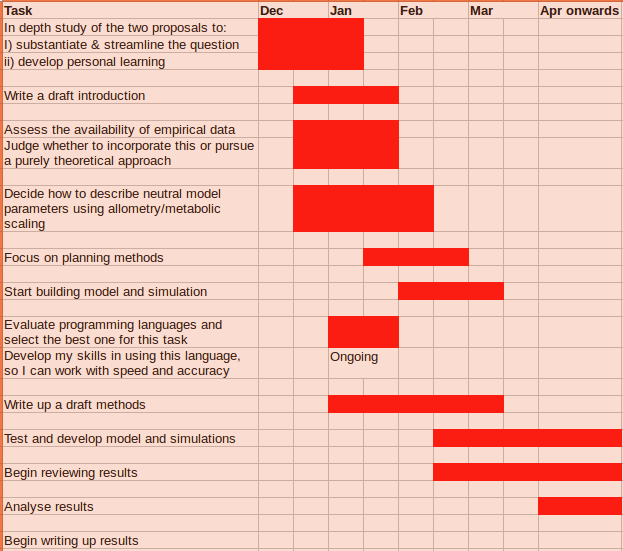
\includegraphics[width=0.8\linewidth]{GANTT.png}
	\caption{Timeline of initial part of project}
\end{figure}

\section*{Budget}
\begin{description}
\item [Printing] - papers for reading; dissertation (\pounds125)
\item [Contingency] - e.g. attending a conference (\pounds375)

\end{description}

\bibliographystyle{apalike}
\bibliography{Biblio2}

\end{document}